%%%%%%%%%%%%%%%%%%%%%%%%%%%%%%%%%%%%%%%%%
% University of Newcastle report 
% LaTeX Template
% Version 1.0 (20/2/19)
%
% This template has been downloaded from:
% http://www.LaTeXTemplates.com
%
% Original author:
% WikiBooks (http://en.wikibooks.org/wiki/LaTeX/Title_Creation)
% Modified by Elsa Slattegard to fit Uppsala university
% Modified by Alex Mendes to fit University of Newcastle
% License:
% CC BY-NC-SA 3.0 (http://creativecommons.org/licenses/by-nc-sa/3.0/)

%\title{Title page with logo}
%----------------------------------------------------------------------------------------
%	PACKAGES AND OTHER DOCUMENT CONFIGURATIONS
%----------------------------------------------------------------------------------------

\documentclass[12pt]{article}
\usepackage[english]{babel}
\usepackage[utf8x]{inputenc}
\usepackage{amsmath}
\usepackage{graphicx}
\usepackage{float}
\usepackage[colorinlistoftodos]{todonotes}
 \usepackage[none]{hyphenat} 
 
\begin{document}

\begin{titlepage}

\newcommand{\HRule}{\rule{\linewidth}{0.5mm}} % Defines a new command for the horizontal lines, change thickness here

\center % Center everything on the page
 
%----------------------------------------------------------------------------------------
%	HEADING SECTIONS
%----------------------------------------------------------------------------------------

\textsc{\LARGE The University of Newcastle}\\[0.5cm]
\textsc{\large School of Electrical Engineering and Computing}\\[1.0cm] % Name of your university/college

\includegraphics[scale=.3]{uon-logo-square.png}\\[1cm] % Include a department/university logo - this will require the graphicx package
\textsc{\LARGE Work Integrated Learning}\\[0.5cm] % Major heading such as course name
\textsc{\large COMP3851A - Semester 2, 2020}\\[0.5cm] % Minor heading such as course title

%----------------------------------------------------------------------------------------
%	TITLE SECTION
%----------------------------------------------------------------------------------------

\HRule \\[0.4cm]
{ \huge \bfseries Interim Report}\\[0.4cm] % Title of your document
\HRule \\[1.5cm]
 
%----------------------------------------------------------------------------------------
%	AUTHOR SECTION
%----------------------------------------------------------------------------------------

\begin{minipage}{1.0\textwidth}
\begin{flushleft} \large
\emph{Authors:}\\
Benjamin \textsc Howard - 3201174\\ % Student 1
Damanjit \textsc Gill - 3285971 \\ % Student 2
Yiming \textsc Yan - 3271479 \\%Student 3
\end{flushleft}
\end{minipage}\\[2cm]

% If you don't want a supervisor, uncommon the two lines below and remove the section above
%\Large \emph{Author:}\\
%John \textsc{Smith}\\[3cm] % Your name

%----------------------------------------------------------------------------------------
%	DATE SECTION
%----------------------------------------------------------------------------------------

{\large \today}\\[2cm] % Date, change the \today to a set date if you want to be precise

\vfill % Fill the rest of the page with white space

\end{titlepage}

\section{Project Title} %20 words
 \paragraph{Program Advisory tool assisting students to find the most suitable pathway to complete their degree.}


\section{Research Background}%1000 words
 \paragraph{The objective of the program advisory tool is to help students find a way to complete their degree at any stage of their studies. The project is undertaken as the focus of a collaborative task by students at the University of Newcastle. The motivating force driving the project is the need for improvement upon the current system of self calculation and human error, so that it is easier for students to plan their degree so it can be completed in a timely manner. By removing this confusion it can also helpful to encourage students who are thinking about attempting a second major or degree.}
  
 \paragraph{ Currently a student needs to refer to the program guide and cross reference a colour coded matrix to a list of courses that are potentially no longer offered, have changed their course code or have been merged into another course that is running in another program. They then need to calculate how many units are required to complete their degree and this can present problems, as the wrong courses can be selected and students enrol in courses where they do not have the assumed knowledge or prerequisite skills needed.}
  
  \paragraph{The solution to this problem will take shape over the course of 1 year. This time frame should be agreeable as the collective skills of the team are adequate to meet the technical requirements of the projects successful completion.}




\section{Aims} %250 words
%{\color{green} Keep aims clear and succinct. Numbered items can work well. Are aims measurable? Aims must be attached to deliverables. Self learning is not an aim.
%[Assignment Specs - Must be flexible. What if a program structure changes? What if a course code changes (i.e. course is replaced by an equivalent). Or if the list of assumed knowledge for a course changes? Or if the semester where it is offered also changes?
%Must be extendable. What if I want to include a new major? Or an entire new program?
%Must be able to support full-time, part-time and study breaks.
%Must allow the fine-tuning of the schedule, i.e. moving courses around to see how small changes affect the completion.]}

\paragraph{1. This project aims to develop an Advisory tool that students at the University of Newcastle can utilize to perform queries to assist them in choosing the pathway required to complete their degree.} 

\subparagraph{•	The student would be able to interact with the interface, adjust variables, and visualize the requirements needed to complete their degree. The system must allow for changes in the program structure, all changes to courses at that time including codes, replacement courses, assumed knowledge requirements, what semester the course is running. }

\subparagraph{•	The student would be able to add another major or change their major. The system will able to make changes according to that. Students can also select courses manually and then the system will able to check whether subjects are valid or not.}

\subparagraph{•	The students would be able to choose if they want to student full time or part-time and the system will able to change the project plan according to their selections. Furthermore, students can also able to take study breaks and the systems then will develop a new project plan for the students.}

\subparagraph{•	The system will give the fine-tuning of the schedule. The system will able to guide the students on what changes will take place if they want to move to other universities and how changes in courses will affect their degree.}

\subparagraph{•	A database will store the students’ academic and personal data, a privacy policy will be developed to protect the University and students and their information.}


\begin{figure}[]
\centering
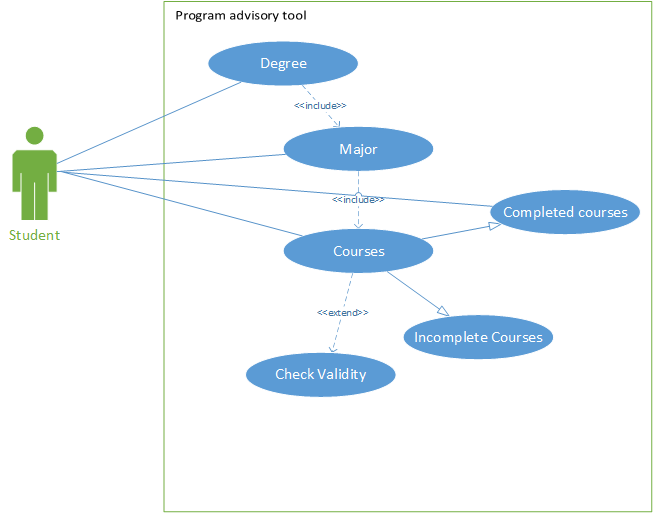
\includegraphics[width = 14cm]{Aims.png}
Figure 1. Use Case Diagram
\end{figure}

\paragraph	{2. In this project, we aim to use additional tools as well. Some of these tools require learning. We aim to use slack and notion for communication, github for sharing code, ‘REACT’ will become the focus of self-learning for the team members, because this is the basic framework for implementing the user interface.~\cite{Spittel2020} 
The Saxon SQL Extension is an auxiliary tool for building databases. Saxon includes a set of extension elements providing access to SQL databases. These are not intended as being necessarily a production-quality piece of software, but more as an illustration of how extension elements can be used to enhance the capability of the processor. Monday.com would be our project management tool to report  progress, the presentation and resolution of problems, and the assignment of tasks will be completed on this tool. Furthermore, for the design of our database, we are going to use the SQL server studio and SAXON will be the tool that will use to link our database to the web pages.~\cite{Kay2020} Also we will aim to create info graphics using Power BI to return results.}

\paragraph{3.	In this project, our tool needs some additional or personal information from the students. To give students certainty that their data is confidential not going to be shared our aim to create a privacy policy and there should be some terms and conditions which will be accepted by students to use the tool. }

\newpage

\section{Methods} %250 words

%Describe the activities undertaken and methods used in your project. Note that this section must be closely related to the aims, i.e. here you must describe the process used to achieve the aims. E.g. for an UI development task, probably there will be some requirement elicitation and initial design, followed by several cycles of implementation, testing and feedback until the interface reaches a stable point. 

\paragraph{Phase 1 - Planning}

\subparagraph{In the planning stage, the team needs to develop a brief project implementation method. The advisory tool will be implemented on the web page.}


\subparagraph{First we have to make a user interface in HTML language using React.The interface  should  include  a  form,  the  form  is  used  to  accept  users degrees, majors and completed courses. The student's degree includes three kinds of ‘bachelor, master and Ph.D’, and the majors should include all majors offered by the university. Users will be asked if they need to add another major.  If another major is included, the core courses of the major will be recalculated. User needs to be separated by semicolons when they input completed courses.  Before submitting,there are some options for students to choose.  Students can choose to take a break from study, they can choose to study full-time or part-time.  After the user completes the input, the information will be provided to the database through the ”Submit” button, and the system will calculate the data and return the best way for the user to graduate.  The interface should also contain some auxiliary tools, like a ”clear” button to clear the user’s input.}

\begin{figure}[h]
\centering
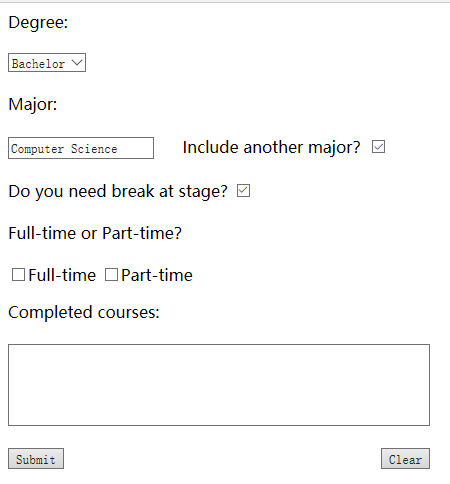
\includegraphics[width=6cm]{./htmldemo.png}\\
Figure 2. User interface prototype.
\end{figure}

\subparagraph{Secondly we have to create a database using SQL server studio to store course information and other content. In the process of designing the database, a privacy policy will be formulated to protect the university and students and their information\\}

\begin{figure}[h]
\centering
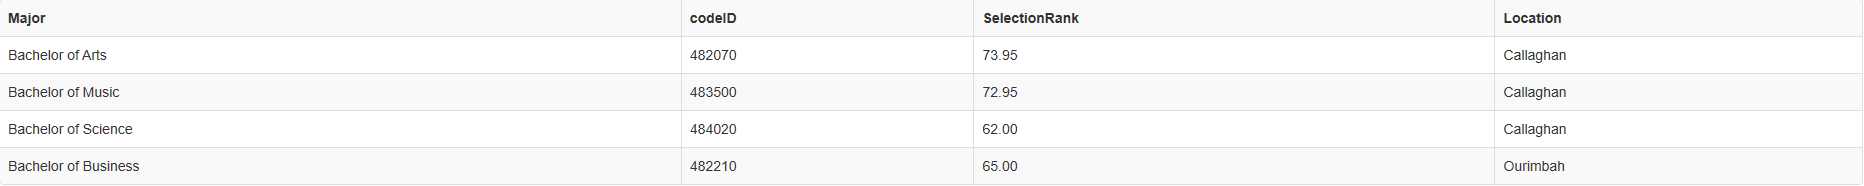
\includegraphics[width=14cm]{./sqlMajor.png}
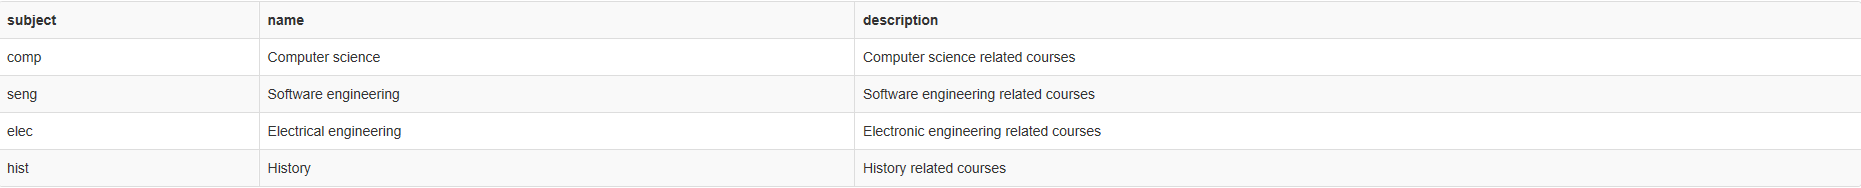
\includegraphics[width=14cm]{./course.png}
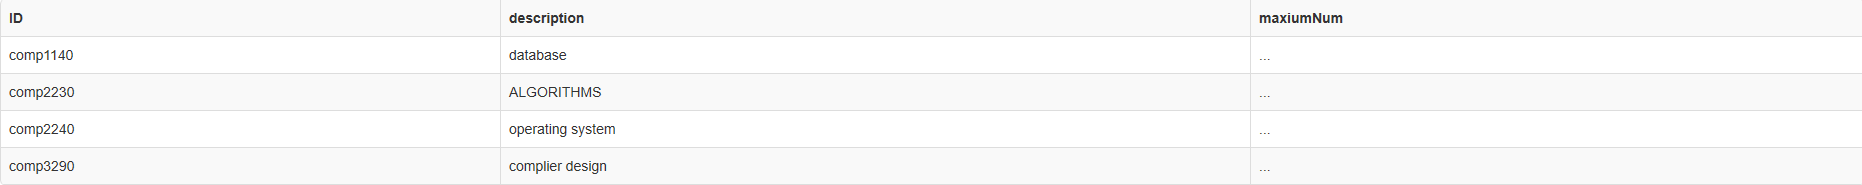
\includegraphics[width=14cm]{./comp.png}
Figure 3. Database table
\end{figure}

\subparagraph{Thirdly we have to write JavaScript functions to solve the problem: Students submit majors and degrees to obtain all core courses; If a course is not offered in the current semester, what course should be used instead.}

\paragraph{Phase 2 - Design}

\subparagraph{After completing the planning phase, the team needs to evaluate which tools will be used. React/HTML and JavaScript are required for the web interface and logic design, and SQL is needed for database establishment.}

\subparagraph{Next, the team needs to draw an EER diagram for the database design. The EER diagram is used to determine what tables will be created and how the tables are related to each other.}

\subparagraph{Finally, the team members need to think about which algorithms will be used. For example, when the user clicks the ‘clear’ button, all the entered information will be cleared; If a student wants to change the order of courses, how does system check if it is allowed? If a student does not pass a course, how changes in courses will affect their degree? etc.}

\begin{figure}[h]
\centering
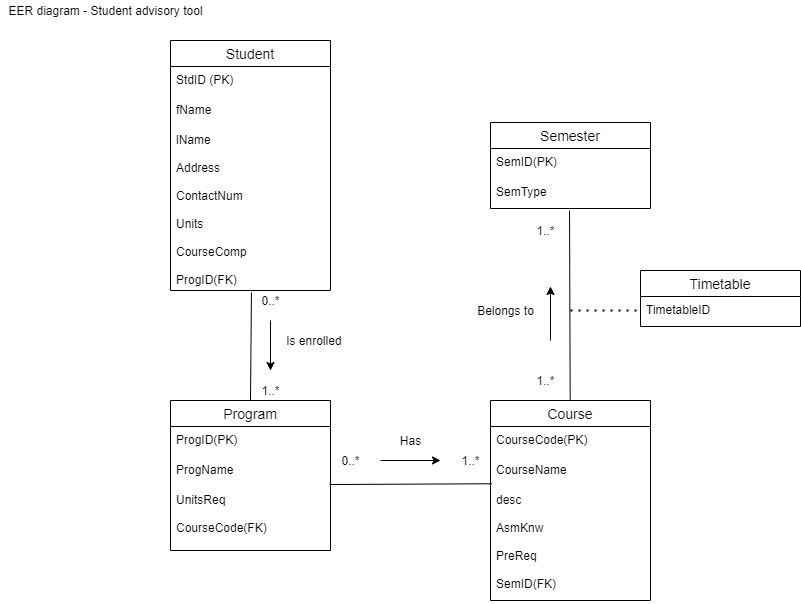
\includegraphics[width=6cm]{./EER.png}\\
Figure 4. Extended Entity Relationship diagram.
\end{figure}

\paragraph{Phase 3 - Build} 

\subparagraph{In the design phase, the team has fully analyzed all logic and technical issues, so in the build phase the team needs to allocate tasks and implement the project design.  Each member needs to report periodically, which has facilitated timely detection of existing problems, and these tools will be used in our build:}

\paragraph{Phase 4 - Implementation}

\subparagraph{'Plan Do Check Act cycle' will be used in Implementation phase.}

\subparagraph{1. Planning stage: Analyze the status quo, find out the existing quality problems and influencing factors, formulate measures to improve quality, put forward an action plan and predict the effect. At this stage, the following questions should be considered repeatedly. Initially the scope will be reduced and a small scale version of the tool will be developed by mapping majors in selected programs before expanding if it tests successfully.}

\subparagraph{Why should these measures be formulated? What purpose will these measures achieve? Where are these measures implemented? When will it be executed? Who is responsible for implementation? What method is used to complete it?}


\subparagraph{2. Do stage: implementation of plans and measures.}

\subparagraph{3.Action stage: Summarize experience and deal with various problems found. Raise unresolved issues. Through inspection, some measures that are not effective, or whose effects do not meet the requirements, and quality problems that have not been resolved are listed as remaining issues and reflected in the next cycle.
With each cycle, the quality of the project will improve. }

\subparagraph{4. Check stage: check the implementation effect of the plan. By doing self-inspection, mutual inspection, process handover inspection, full-time inspection, etc., the implementation results are compared with the predetermined goals, and the implementation results of the plan are carefully checked.}
\newpage

\section{Results}%750 words

%Describe and analyse the results obtained. Again, for the UI development, you can present a screenshot, diagrams, list of functional requirements, etc. Also, please indicate what are the limitations of the experiments, and the implementation itself in terms of performance and flexibility
%– how could it be extended or modified to suit similar, but different projects? Note again, that the results must reference the aims and methods. 
  %We constructed a low-fidelity model for testing according to the reference aims and method.

\paragraph{1. Database}

\subparagraph{1.1 Student Table: It is currently set 'student' have the attributes of ‘name’, ‘ID’, ‘password’, ‘class’, and ‘gender’. ID and password are used for user login, others are user information.}

\begin{figure}[h]
\centering
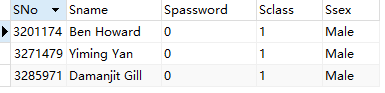
\includegraphics[width=14cm]{./db_student.png}
Student database table
\end{figure}

\subparagraph{1.2 Course Table: It is Currently set 'course has' ‘Number’, ‘Name’, and ‘credit’. Name or Number can be used to query courses, others are course information}

\begin{figure}[h]
\centering
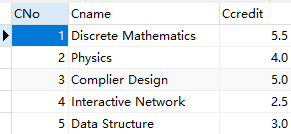
\includegraphics[width=14cm]{./db_course.png}
Course database table
\end{figure}

\newpage

\subparagraph{1.3 Student Course Table: This table associates students with courses. 'SNo' is the student account number, and'CNo' is the course number. The courses selected by the students will be saved to this table.}

\begin{figure}[h]
\centering
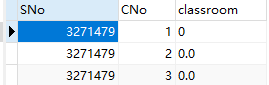
\includegraphics[width=14cm]{./db_studentCourse.png}
Student Course database table
\end{figure}

\newpage

\paragraph{2. User interface}

\subparagraph{2.1 Login in UI: The login interface has two text boxes that accept the username and password, and some logos. It will be validated when the user completes the input. If the verification fails, a message "Incorrect account or password" will pop up. We set the password of the test account as ‘0’ by default, and the user can modify the password after logging in successfully. For the protection of user privacy, the password entered by the user will be replaced by asterisks, and the link to the privacy policy needs to be viewed and agreed upon before validating the the user password, a message of 'please read and agree to privacy policy before proceeding' will appear.}

\begin{figure}[h]
\centering

\includegraphics[width=14cm]{./UI_login.png}
User login in page
\end{figure}

\newpage

\subparagraph{2.2 Homepage UI: The homepage is used to post announcements. The navigation bar will always be on the left. The navigation bar has five parts, namely, avatar, course selection, view the courses user has selected, view student information and exit.}

\begin{figure}[h]
\centering
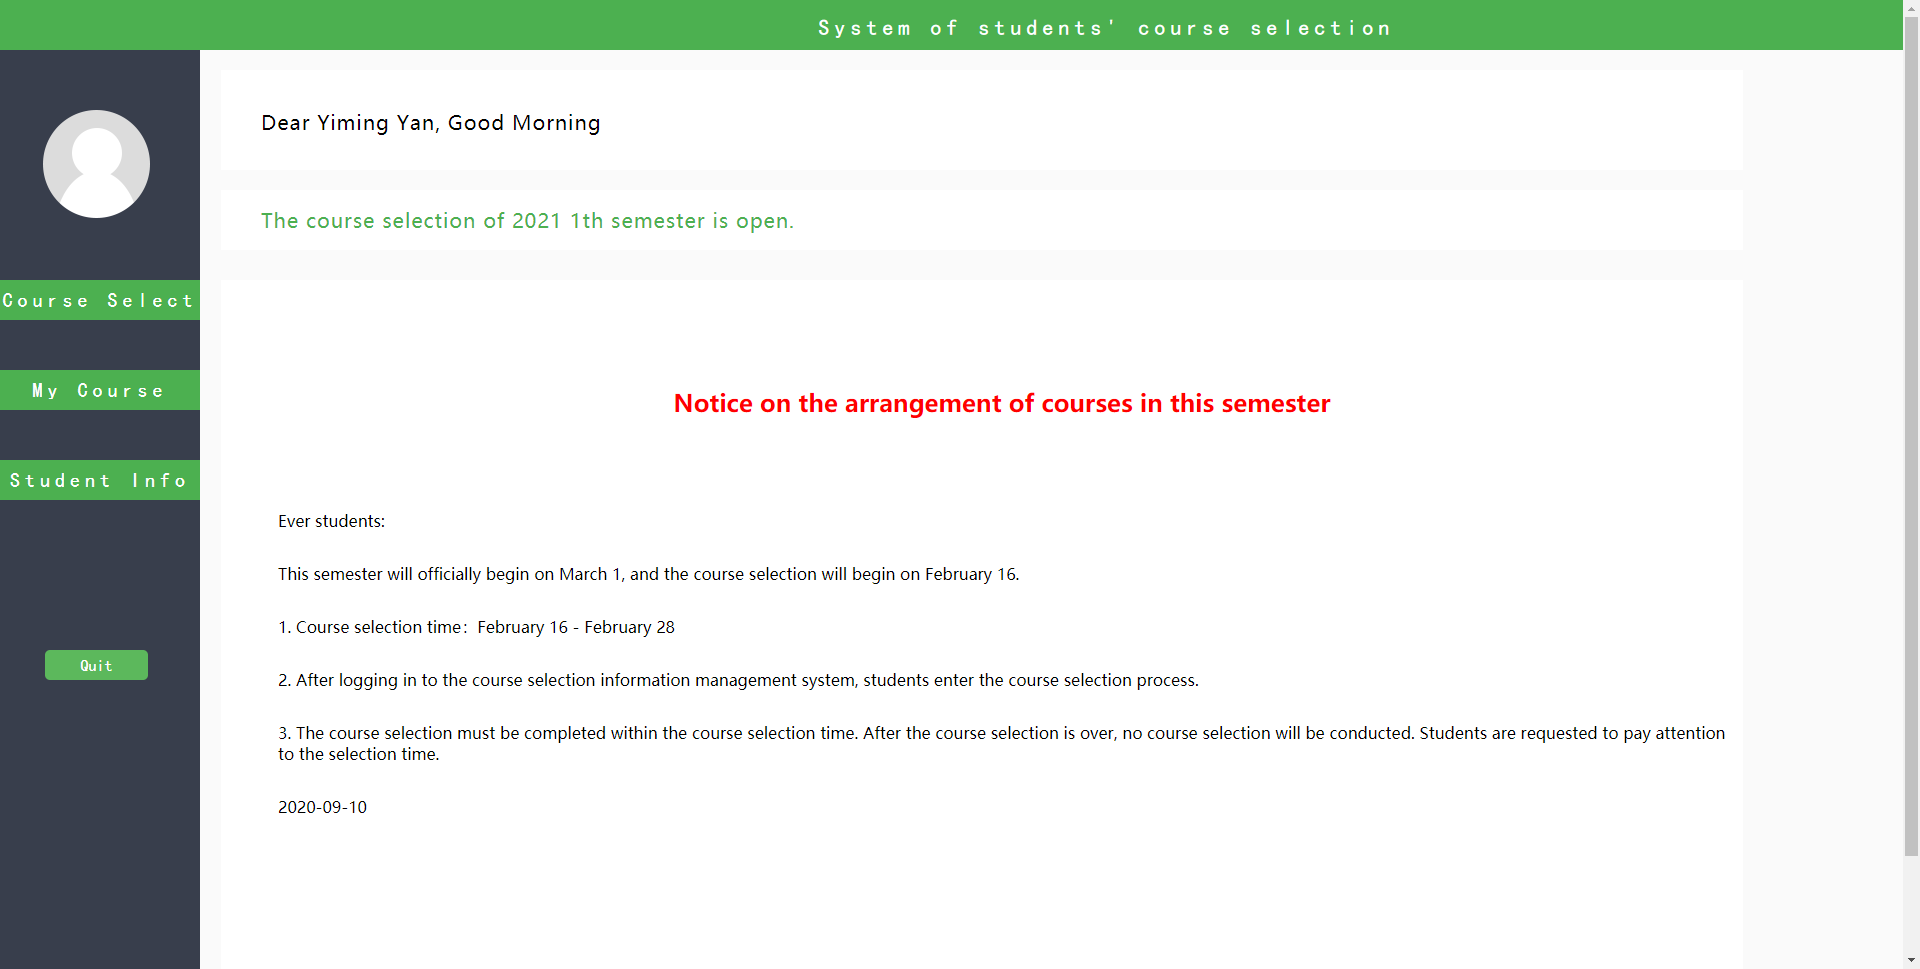
\includegraphics[width=14cm]{./UI_homepage.png}
Homepage
\end{figure}
\newpage

\subparagraph{2.3 Course Selection UI: This is the course selection page. We only inserted 10 courses for testing, so the course search function is currently not implemented. When there are enough courses, we can search according to the code or name of the course. After selecting the ‘selection’ check-box and submitting it, the back-end will update the students with the selected courses (update sc table), and users can query their own courses through the ‘selected courses’. If you click the ‘cancel’ button, all check-boxes will be recover. However, computing the best graduation path for students has not yet been realized. Our idea is to obtain all the courses that students need to pass based on the student's information, then screen out the failed courses and allocate them to each semester.}

\begin{figure}[h]
\centering
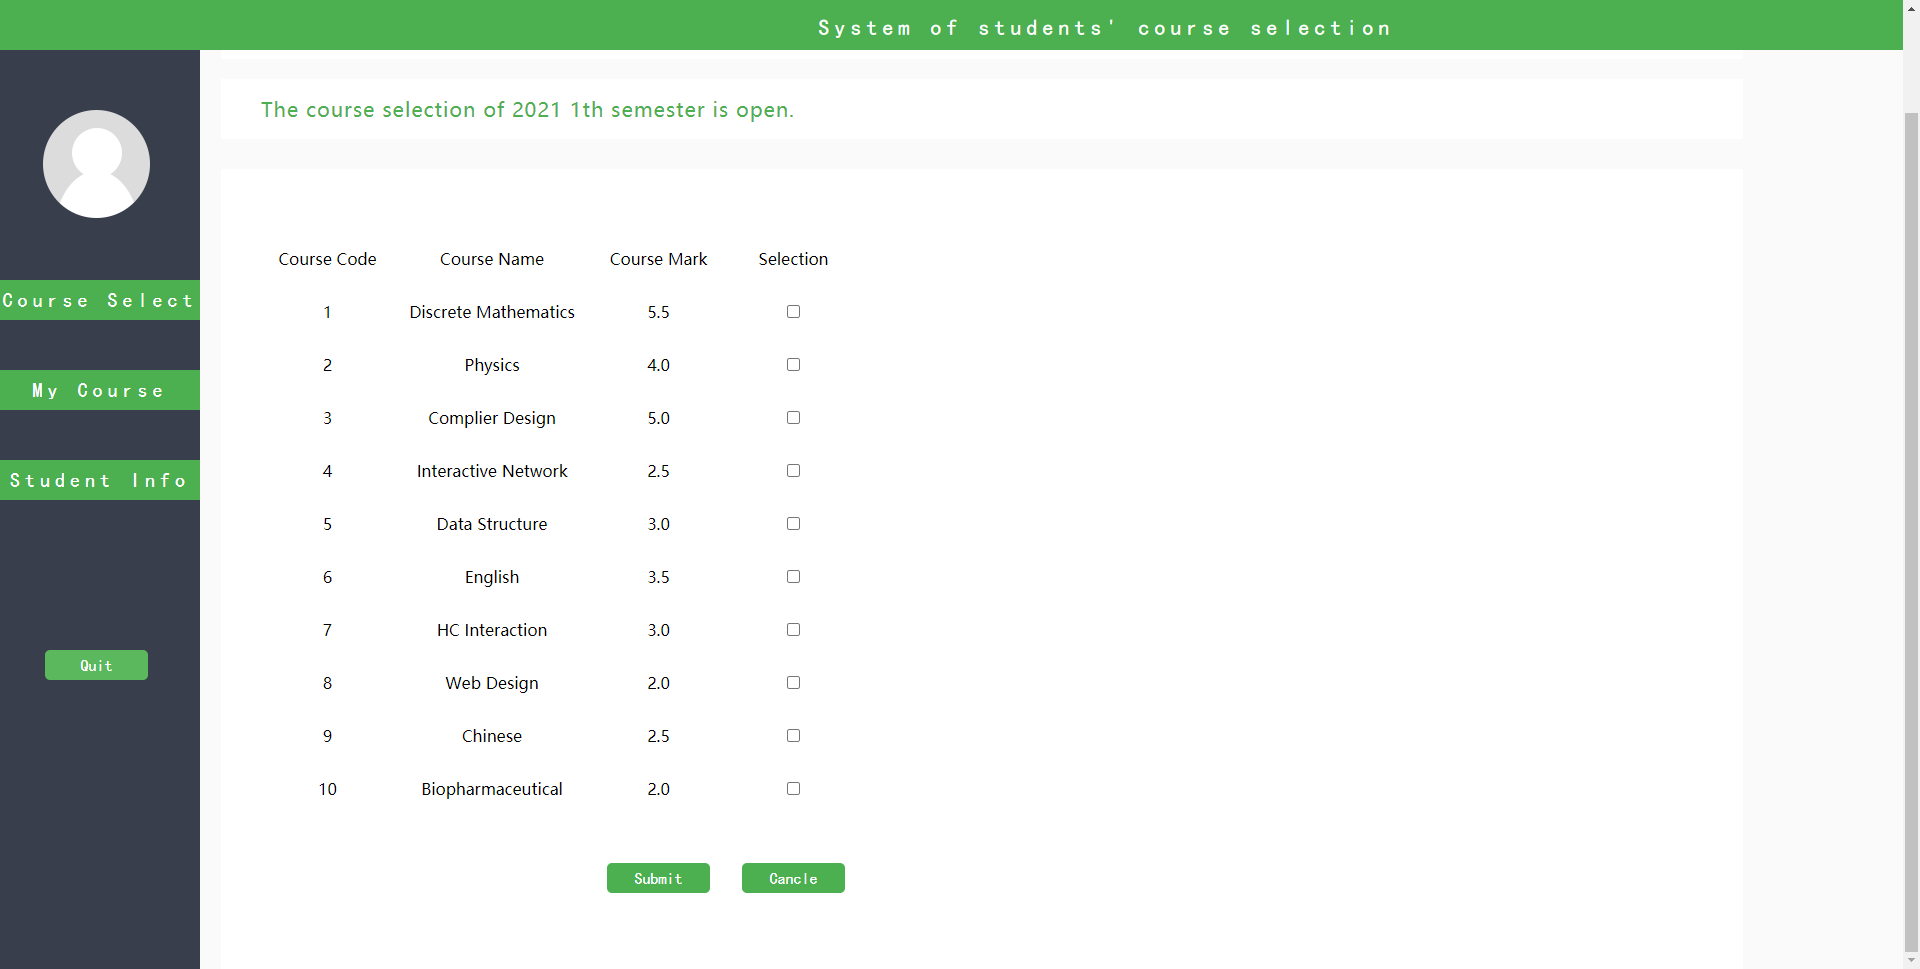
\includegraphics[width=14cm]{./UI_cs.png}
Course Select page
\end{figure}
\newpage

\subparagraph{2.4 Selected Courses UI: On the selected course page, the user can see the currently selected course, and the interface provides some basic information about the course. Students can do drop course.}

\begin{figure}[h]
\centering
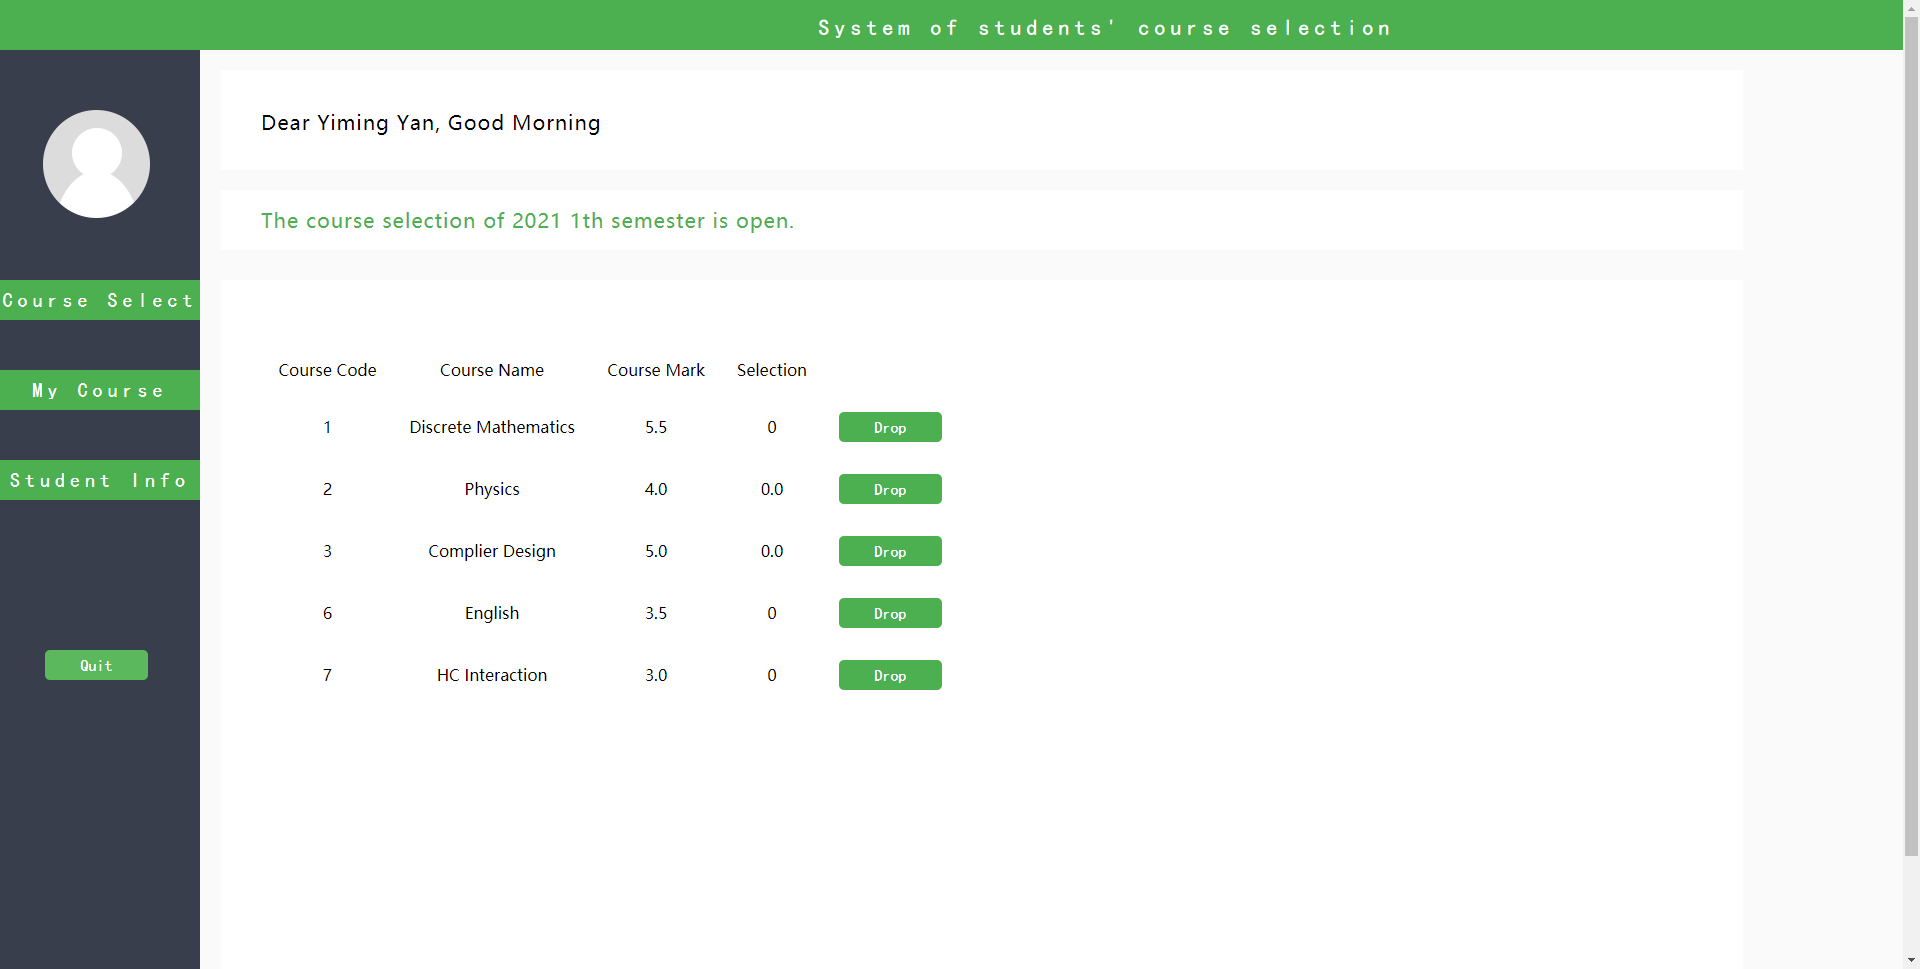
\includegraphics[width=14cm]{./UI_mc.png}
Selected Courses page
\end{figure}

\newpage

\subparagraph{2.5 Student Information UI: This page is for browsing students’ personal information. Student information includes: ‘student name’, ‘student account’, ‘password’, ‘gender’, ‘class’, and ‘credits’. Students can modify basic personal information here, including name, password, gender, etc. Other information cannot be modified because the student account is constant, and other information is calculated based on the student's course. }

\begin{figure}[h]
\centering
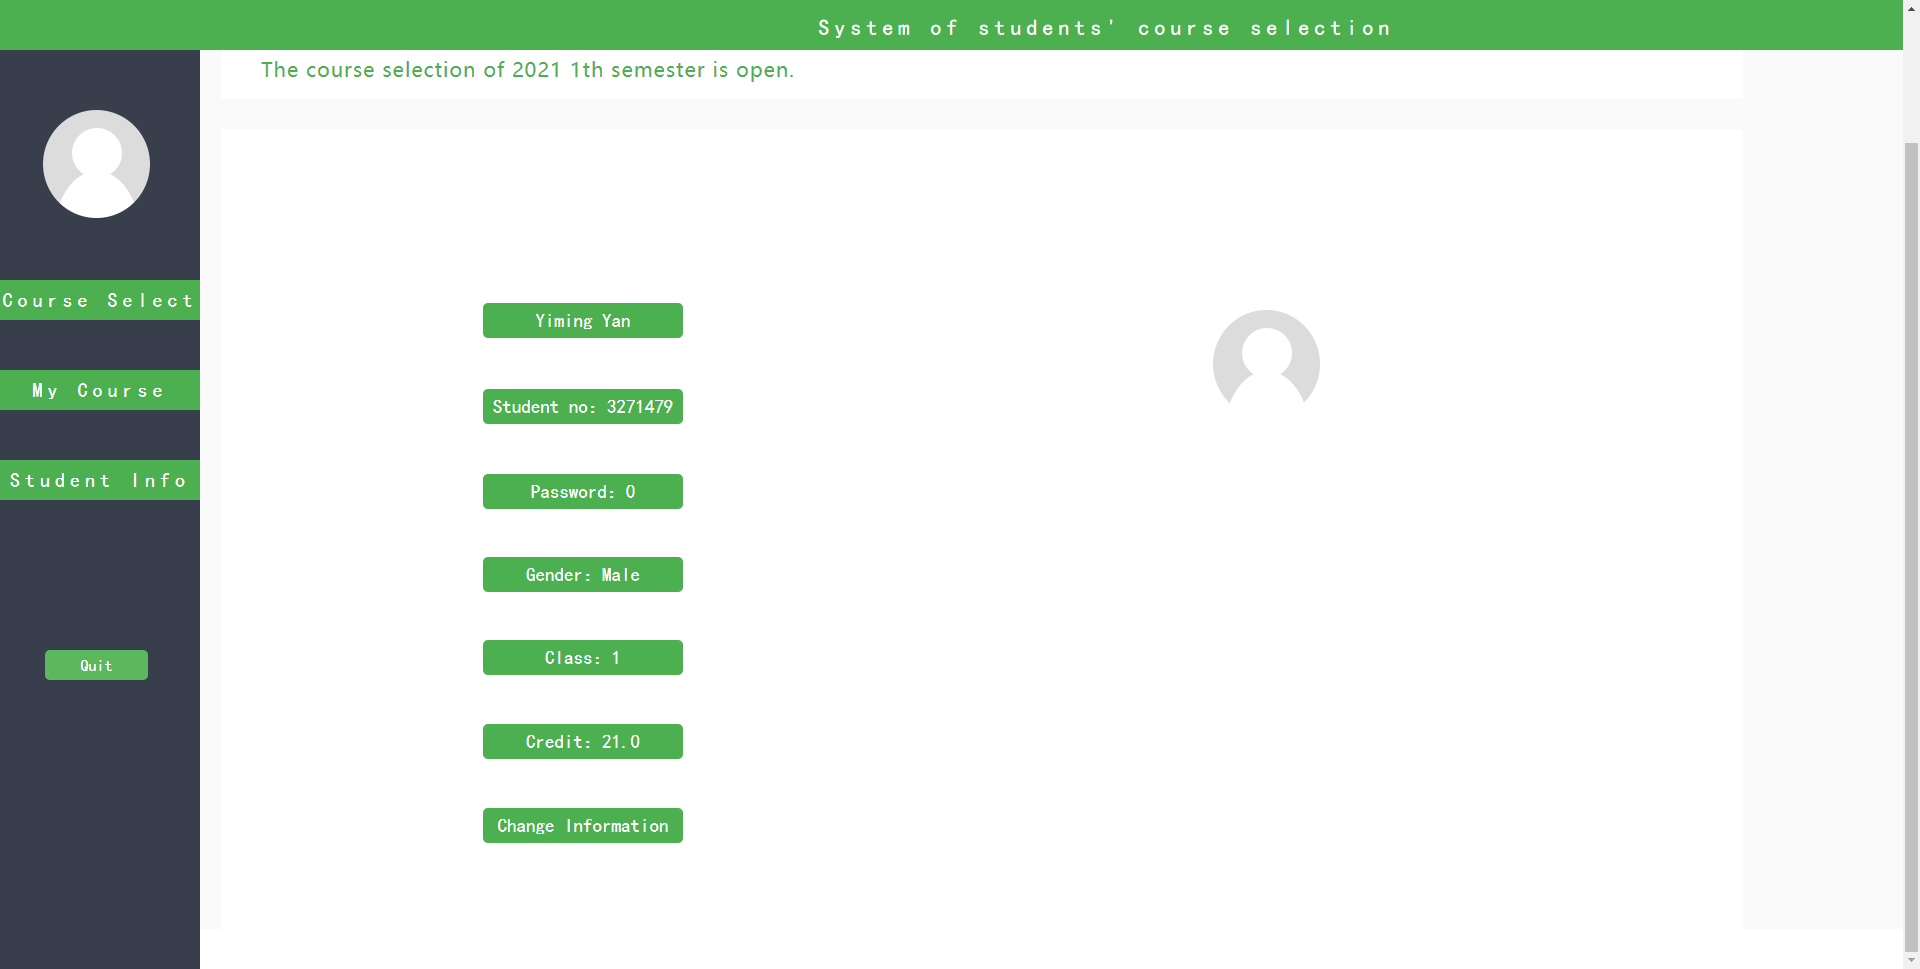
\includegraphics[width=14cm]{./UI_si.png}
Student Information page
\end{figure}

\newpage
 
\paragraph{3. Summary: Our team has completed the construction of the project framework. }

\paragraph{List of currently implemented functions:}
\subparagraph{1. Connect the database to the program}
\subparagraph{2. User login and logout}
\subparagraph{3. Check the validity of the user}
\subparagraph{4. Check all courses}
\subparagraph{5. Query user selected courses}
\subparagraph{6. Drop the course selected by the student}
\subparagraph{7. Query student personal information}
\subparagraph{8. Update student personal information}

\paragraph{Unrealized functions:}
\subparagraph{1. Supplement of course information. (For example, the premise of learning a certain course, the semester of a certain course.)}
\subparagraph{2. Allow students to choose full-time, part-time or rest.}
\subparagraph{3. Allow students to fill in a new major.}
\subparagraph{4. Allow students to fine-tune the schedule.}
\subparagraph{5. Students are required to provide completed courses, and the back-end feedbacks the courses that students need to complete according to the information, and calculates the best graduation path.}
\subparagraph{6. Database functionality is not operating to requirements, the database running in app is for demonstration purposes only.}
\subparagraph{Link to privacy policy and validation button at login page.}

\newpage

\paragraph{Our program still has some limitations: students cannot return after leaving the homepage, courses cannot be allocated according to major types, the database design and functionality is limited due to selecting appropriate check constraints that are compatible with the framework design, by using agile methods to continually improve the database structure these limitations can be over come by trial and error when creating more appropriate queries,  these are the main improvement targets in the future. 
\para The performance of this program is very high because the code is very concise, so the system responds quickly. The flexibility of the program is relatively high, because the code is written norms for easy reading and modification. Each function is implemented by a separate class, and all functions can be easily understood. When adding or deleting functions, it will basically not affect the normal use of other functions. For example, I currently need to add a course attribute (courseNo), I only need to find the construction class of "course", and add this attribute in the constructor, and write setter and getter for the attribute. Then rebuild the course schedule in the database, and then call the courseNo of the course. Or I want to implement a function to query the number of people selected for a course in order to manage the course. I can set a variable ‘count’ to record the selection or drop of each course. Then write a function to accept the course number entered by the user and return the ‘count’ corresponding to this course. Course administrators can better manage courses.}

\newpage


\section{Ethics } %250 words
%Describe any ethical issues that have arisen during the project and potential future ones, and how the group plans to mitigate them. 

\paragraph {Data Security - The application will collect and store data from students, therefor the privacy of user data must be protected and kept confidential. The privacy policy will protect students and clearly document the expectation of all parties who use the application.
\par The application will not progress past the login screen until the privacy policy is viewed and the user agrees to them, they will clearly outline what the policy is about, who the team represents, what information is collected, how it is collected and used. It will also inform the user how long the data is stored and where it is stored to avoid discarding every session afterwards. It will also outline the users rights under the relevant legislation, how to access the data and the process required to delete it, how to complain to the regulatory bodies. It will discuss security measures in place, the use of cookies and social plugins. The policy will be regularly updated and information pertaining to this process will be available to the user. Lastly there will be contact details for the group(company) where questions about the privacy policy and Application can be answered.The formation of the privacy policy framework was based upon researching similar such policies noteably   Terms and conditions should also outline the users responsibilities and protect the University from liability and a link to them is below the login page but does not prevent access to the application.~\cite{Ladwig202050}}
\newpage


\bibliographystyle{elsarticle-num}
\bibliography{mybibfile}

\section*{Statement of individual contribution}
\emph{Contribution:}\\
Benjamin \textsc Howard - Title, background, excpected outcomes(limitations), Ethics, Referencing, Proof reading, EER,   \\ % Student 1
Damanjit \textsc Gill - Aims, expected outcomes, required tools research, Use case diagram.\\ % Student 2
Yiming \textsc Yan -  Result\\%Student 3



\section*{Appendix}
\begin{figure}[h]
\centering
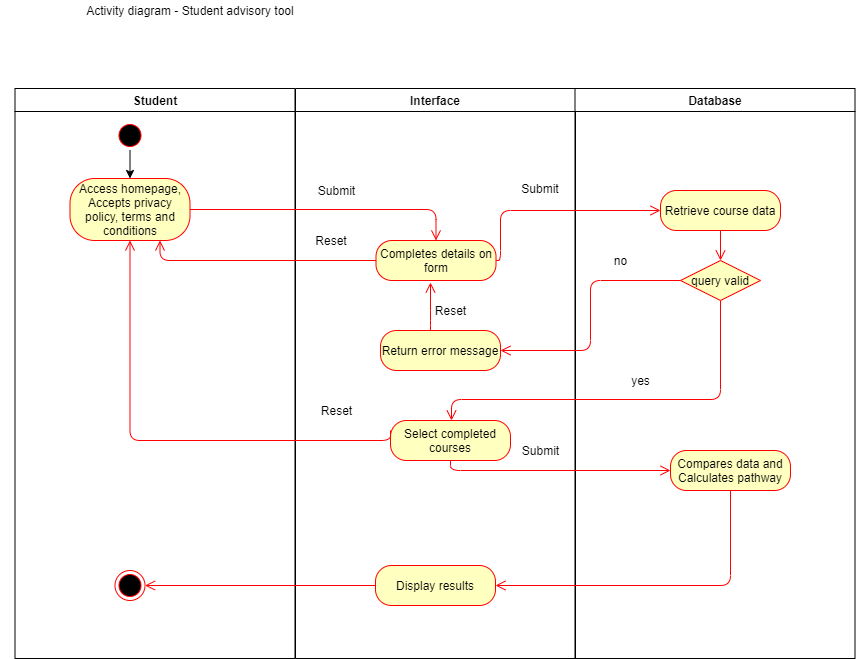
\includegraphics[width=6cm]{./ActivityDiagram.png}\\
Figure a Activity diagram for advisory tool.
\end{figure}



\begin{figure}[h]
\centering
\label{fig:comms}
\end{figure}
\end{document}



